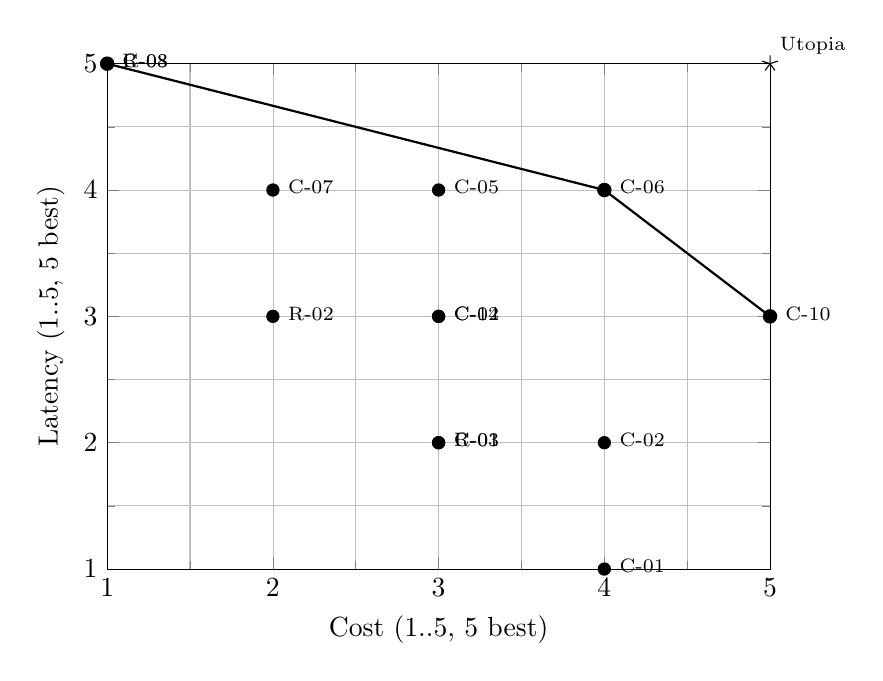
\begin{tikzpicture}
\begin{axis}[
  width=10cm,
  height=8cm,
  xmin=1, xmax=5,
  ymin=1, ymax=5,
  xtick={1,2,3,4,5},
  ytick={1,2,3,4,5},
  xlabel={Cost (1..5, 5 best)},
  ylabel={Latency (1..5, 5 best)},
  grid=both,
  major grid style={line width=0.2pt},
  minor tick num=1,
  clip=false, % so labels can sit outside
]

% --- All candidates: (x,y) with label
% Format: (x,y)[label]
\addplot[
  only marks,
  mark=*,
  mark size=2.2pt,
] coordinates {
  (4, 1) [C-01]
  (4, 2) [C-02]
  (3, 2) [C-03]
  (3, 3) [C-04]
  (3, 4) [C-05]
  (4, 4) [C-06]
  (2, 4) [C-07]
  (1, 5) [C-08]
  (5, 3) [C-10]
  (3, 3) [C-12]
  (3, 2) [R-01]
  (2, 3) [R-02]
  (1, 5) [R-03]
};

% Labels for all points
\addplot[
  only marks,
  mark=none,
  nodes near coords,
  point meta=explicit symbolic,
  nodes near coords style={
    font=\scriptsize,
    anchor=west,
    xshift=2pt,
    yshift=1pt,
  },
] coordinates {
  (4, 1) [C-01]
  (4, 2) [C-02]
  (3, 2) [C-03]
  (3, 3) [C-04]
  (3, 4) [C-05]
  (4, 4) [C-06]
  (2, 4) [C-07]
  (1, 5) [C-08]
  (5, 3) [C-10]
  (3, 3) [C-12]
  (3, 2) [R-01]
  (2, 3) [R-02]
  (1, 5) [R-03]
};

% --- Pareto front: list in the order you want connected
\addplot[
  thick,
  mark=*,
  mark size=2.2pt,
] coordinates {
  %(4, 1) [C-01]
  %(4, 2) [C-02]
  %(3, 2) [C-03]
  %(3, 3) [C-04]
  %(3, 4) [C-05]
  %(2, 4) [C-07]
  (1, 5) [C-08]
  (4, 4) [C-06]
  (5, 3) [C-10]
  %(3, 3) [C-12]
  %(3, 2) [R-01]
  %(2, 3) [R-02]
  %(1, 5) [R-03]
};

% --- Utopia point (5,5) as a star
\addplot[
  only marks,
  mark=star,
  mark size=3.0pt,
] coordinates {(5,5)};

\node[font=\scriptsize, anchor=south west] at (axis cs:5,5) {Utopia};

\end{axis}
\end{tikzpicture}
